\chapter{Invisible CAPPCHA}\label{chapter:InvisibleCAPPCHA}
The \textit{Invisible CAPPCHA} is an evolution of CAPPCHA, in terms of usability\cite{Invisible_CAPPCHA}. The main difference with respect to CAPPCHA is that the challenge isn't explicitly submitted to the user but it's hidden behind the PIN authentication phase. This type of challenge works only on smartphones as its ancestor but it's very important to understand how data, obtained by the sensors, could be exploited during the authentication phase.\\
Invisible CAPPCHA is a method developed in 2018 and based on motion side-channel of mobile devices and it's very effective as support of Password-based authentication methods. The main steps, followed by this CAPTCHA, are:
\begin{enumerate}
\descItem{Motion detection}{in this phase the micro-movements of the device, generated by the interaction of the user with the touch-screen, are evaluated by the \textit{Secure Element} (\textit{SE})}
\descItem{Communication between Client and Server}{in this phase the credentials are shared with the remote Service Provider}
\end{enumerate}
The following sections will analyse this steps highlighting some peculiarities of Invisible CAPPCHA that will be used or modified to develop AcCAPPCHA, a CAPTCHA based on microphone sensors.

\section{Motion detection}
In this first phase, Invisible CAPPCHA exploits the accelerometer of the mobile device. It detects the acceleration over the three axis in g-force units, as a sequence of vectors over time:
$$\{ A_i\}_{i=1}^{n} = \{ (a_1^x, a_1^y, a_1^z), ..., (a_n^x, a_n^y, a_n^z)\}$$
This type of side-channel information from embedded accelerometer has been exploited in different attacks for the single and double tap detection. These attacks analyse the accelerations over the z-axis by comparing them to some thresholds and some timing conditions.\\
In Invisible CAPPCHA, the side-channel information is stored on the memory of the mobile device. Depending on the device, a smartphone built-in vibration can be generated along Z axis or along more than one axis (see \myref{Figure}{inv:vibration}). At the contrary a finger tap event is defined by strong accelerations on Z-axis but also similar one to the other (see \myref{Figure}{inv:tap}).\\
In Invisible CAPPCHA, the difference between built-in vibration and tap acceleration is evaluated by a simple algorithm. It relies on negative and positive peaks, that are detected by comparing acceleration along Z axis with predefined thresholds. The differences between the tap accelerations and the vibrations is the main characteristic that guarantees user's tap cannot be simulated by a bot using the vibration motors.\\
Another important requirement, to prevent a bot attack, is that Invisible CAPPCHA uses a Secure Element that embedded the accelerometer of the device. In this way malicious code can't access to the sensor. Nowadays there exists a smart card, called SIMSense, that already integrates motion sensor and embeds it in a Secure Element.\\
\begin{figure}[h]
     \centering
     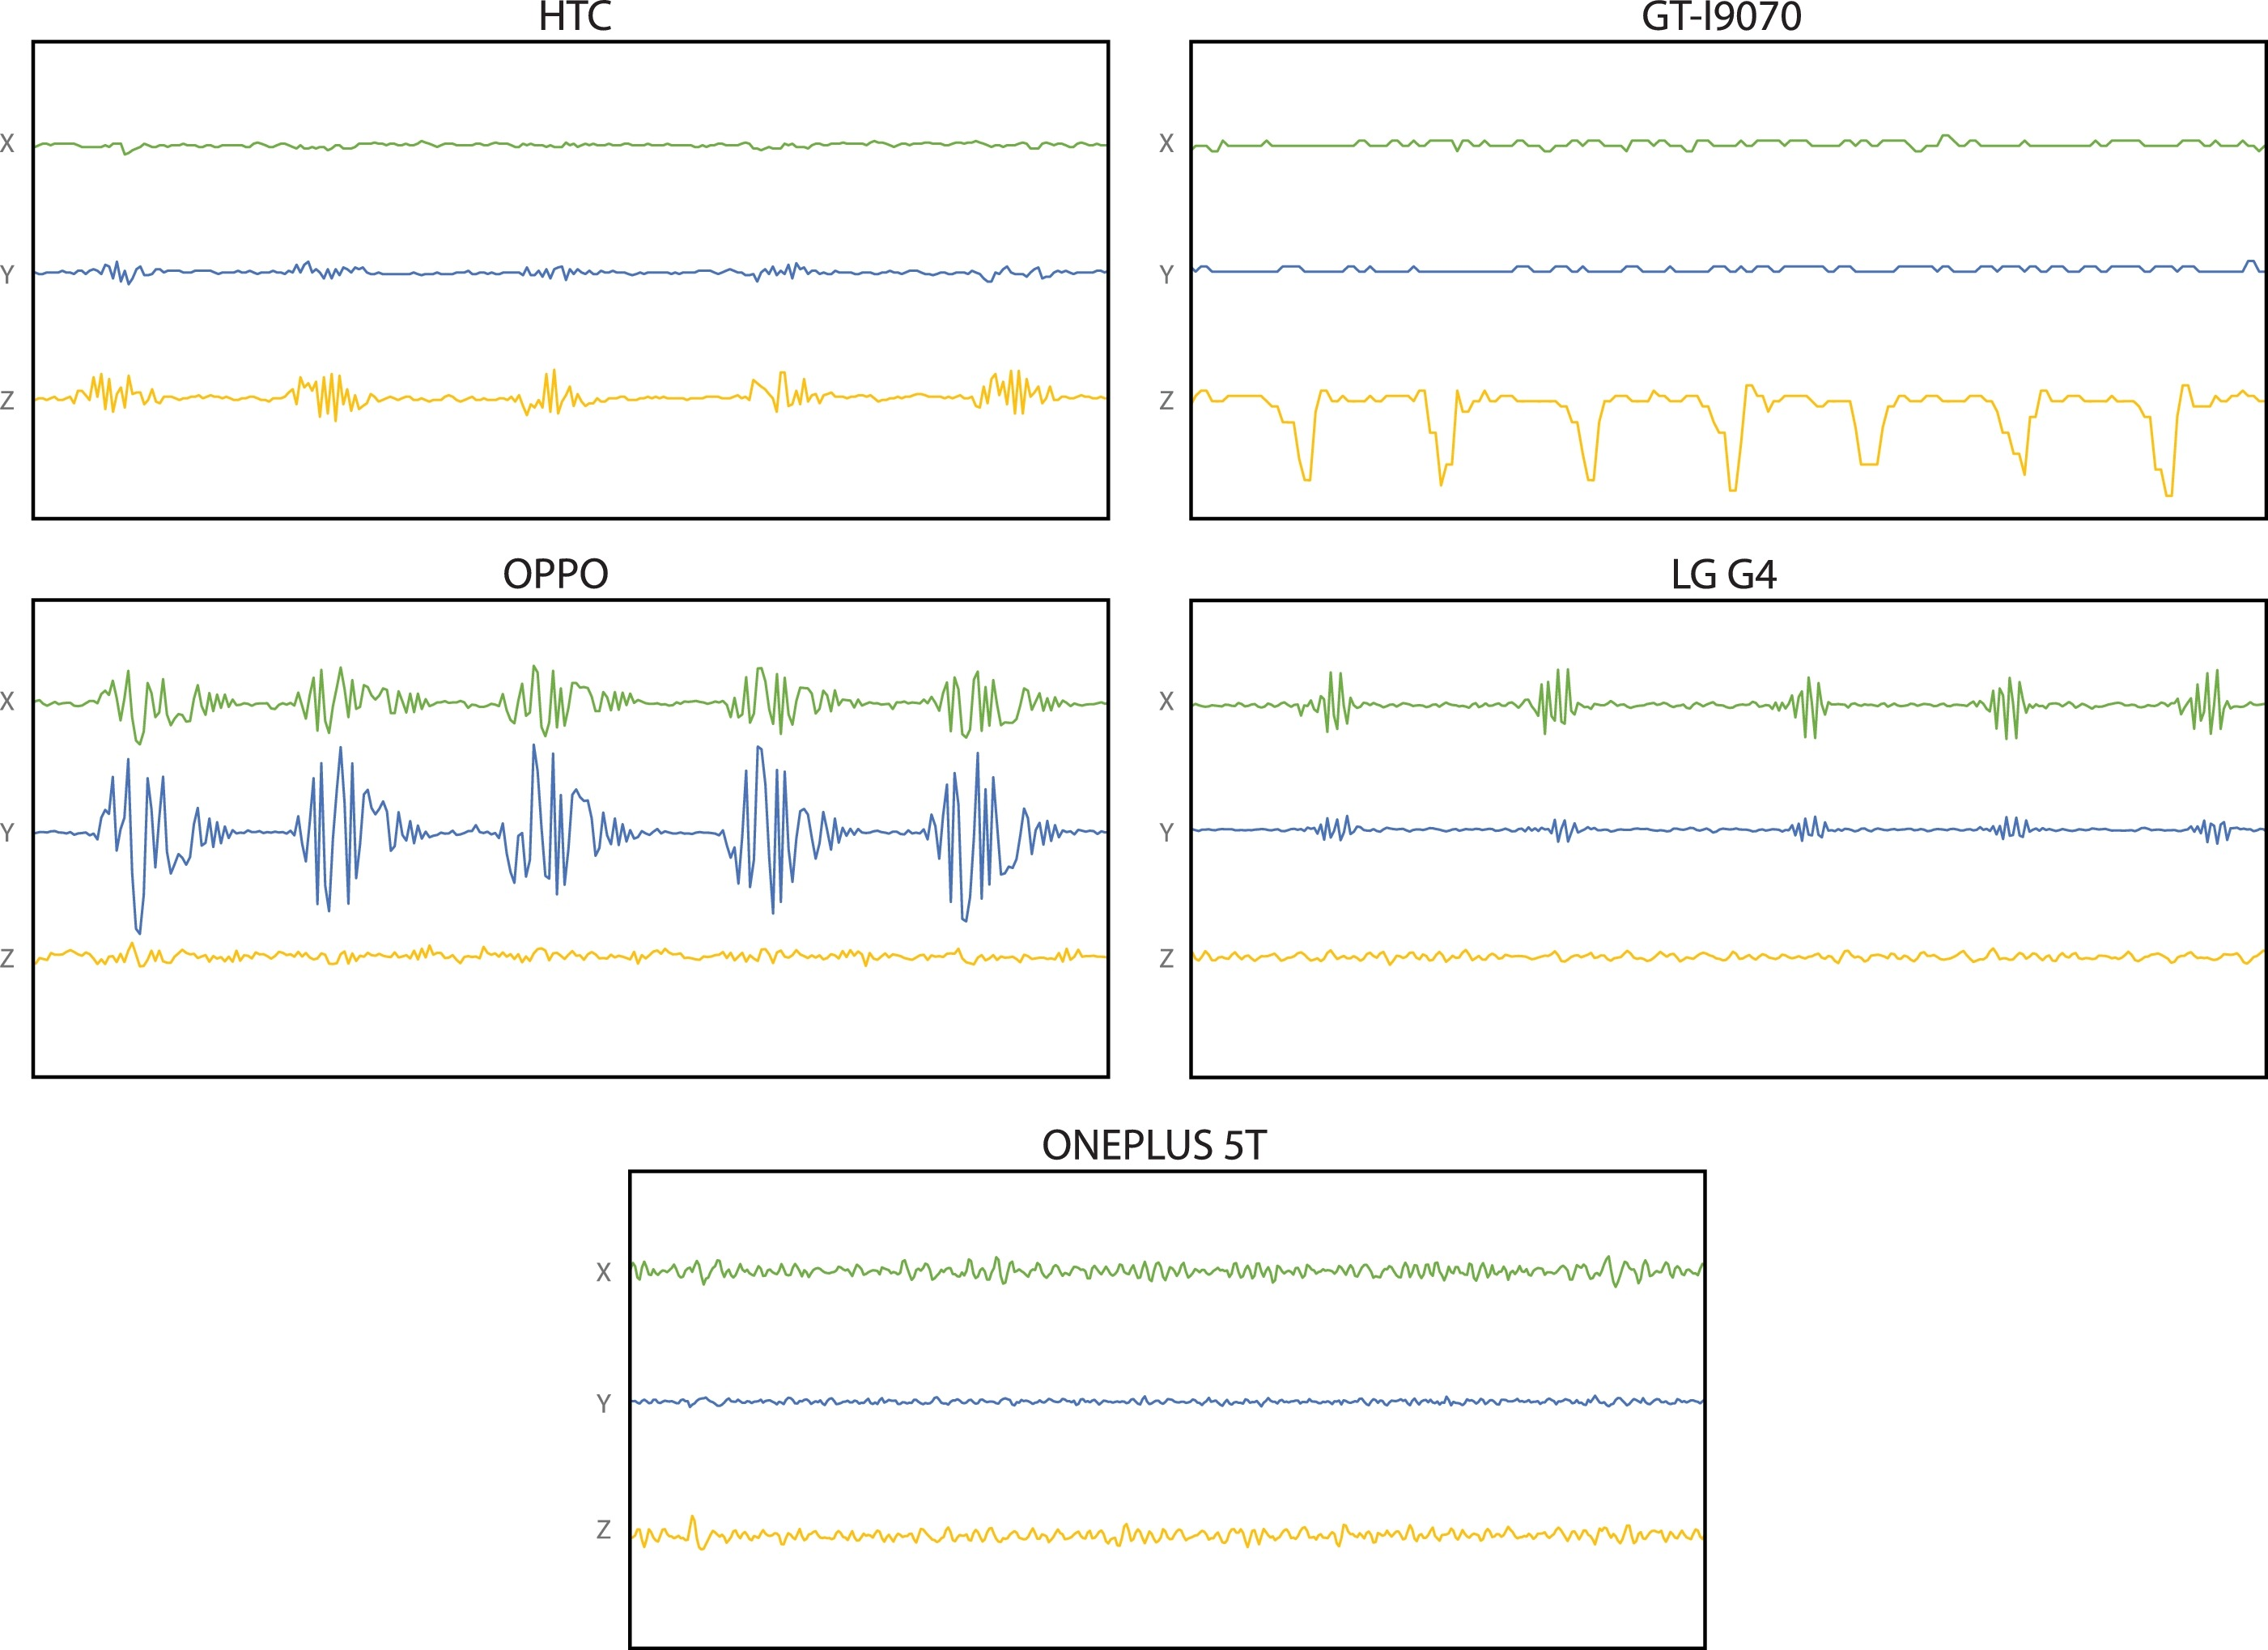
\includegraphics[width=.8\linewidth]{Images/InvisibleCAPPCHA/vibration}
     \caption{\footnotesize{Example of accelerations caused by smartphone built-in vibration.}}\label{inv:vibration}
\end{figure}
\begin{figure}[h]
     \centering
     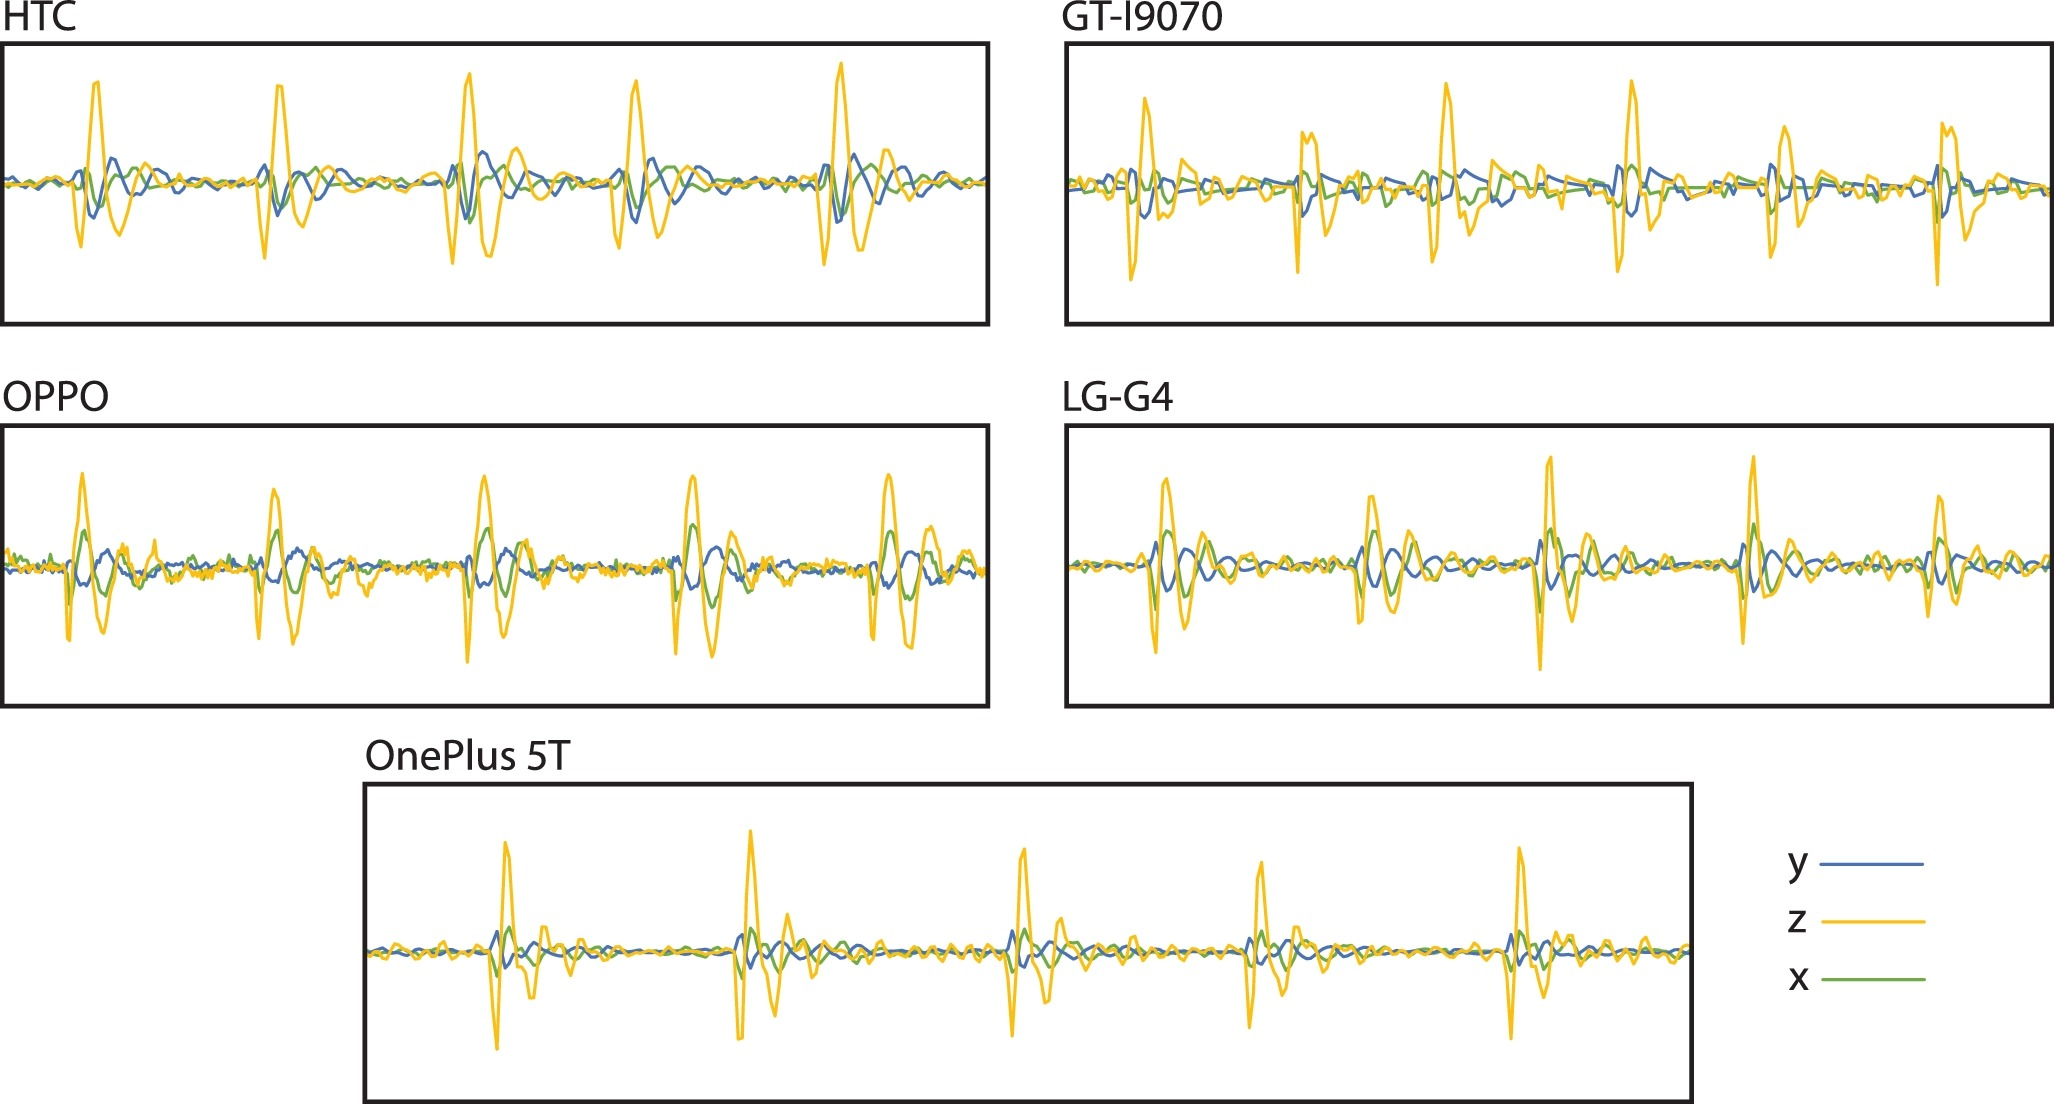
\includegraphics[width=.8\linewidth]{Images/InvisibleCAPPCHA/tap}
     \caption{\footnotesize{Example of accelerations caused by finger tap detection.}}\label{inv:tap}
\end{figure}


\section{Communication between Client and Server}\label{inv:communication}
When the user fills a form or provides other information to a cloud application/service, the Secure Element checks if a micro-movement is measured when a user tap is detect. If this happens the input inserted by user is considered valid, or rather generated by a human, otherwise the algorithm tells that the input was generated by a bot.\\
An extra message, that tells if the task was performed by a user or not, is sent to the server side. The integrity of this message is guaranteed by the Secure Element, that can be equipped with a digital signature. The identity of the device can be associated to the message sent and then it can be checked and verified. The Secure Element signs the verification message through ECDSA.

\subsection{Elliptic Curve Digital Signature Algorithm (ECDSA)}
The elliptic cryptography works similarly to RSA but it uses smaller keys. The signature algorithm with elliptic curves is divided in two phases, like the one based on RSA. Considering two users, Alice and Bob, ECDSA phases are explained in the following lines:
\begin{itemize}
\descItem{Sign generation}
{If Alice wants to send a message, protected with digital sign, to Bob, they need to share the following parameters \textit{(curve, G, n)}: \textit{curve} is the equation of an elliptic curve, \textit{G} is the base point of prime order on the curve and \textit{n} is the multiplicative order of \textit{G} for which $n\; x\; G = O$ ($x$ is the scalar multiplication of a point of the curve).
Alice generates a private key $d_A$ in the range $[1, n-1]$ and a public key $Q_A=d_A\; x\; G$. Alice needs to perform \myref{Algorithm}{inv:ECDSA_sign} to sign a message $m$.
\begin{algorithm}[h]
\DontPrintSemicolon\footnotesize
\KwIn {$\mathtt{m}$= message to be signed}
\KwOut {$\mathtt{(r,s)}$= digital sign}
\BlankLine
$e\gets HASH(m)\;$where \textit{HASH} is an hash function (e.g. SHA-2)\;
\BlankLine
$z \gets$ string composed by the $L_n$ most left bits\;
$\;\;\;\;\;\;\;$where $L_n$ is the bit length of the group of order $n$\;
$r\gets 0$\;
$s\gets 0$\;
\BlankLine
\While{$r=0\;mod\;n$ or $r=0\;mod\;n$}{
	\BlankLine
	$k\gets RANDOM([1,n-1])$\;
	\BlankLine
	$(x_1, y_1)=k\;x\;G$ of the elliptic curve\;
	\BlankLine
	$r\gets x_1\; mod\; n$\;
	\BlankLine
	{$s\gets k^{-1}(z+rd_{A})\; mod\; n$}
	\BlankLine
}
\caption{Sign generation.}\label{inv:ECDSA_sign}
\end{algorithm}
}
\descItem{Sign verification}
{Bob wants to verify the digital signature sent by Alice. To do it, he needs to apply in order \myref{Algorithm}{inv:ECDSA_key_verify} and \textbf{\ref{inv:ECDSA_verify}}.\\
\begin{algorithm}[h]
\DontPrintSemicolon\footnotesize
\KwIn {$\mathtt{Q_A}$= public key to be verified}
\KwOut {$\mathtt{check}$= true if public key is correct}
\BlankLine
$\mathtt{check}\gets true$\;
\BlankLine
$\setminus\setminus$Valid coordinates\;
\If{$Q_A=O$}
{	
$\mathtt{check}\gets false$\;
}
\BlankLine
$\setminus\setminus$Element of the curve\;
\If{$Q_A\;\in$ curve}
{	
$\mathtt{check}\gets false$\;
}
\BlankLine
$\setminus\setminus$Correctness of order\;
\If{not $n\;x\;Q_A=O$}
{	
$\mathtt{check}\gets false$\;
}
\caption{Verification that public key is on the elliptic curve.}\label{inv:ECDSA_key_verify}
\end{algorithm}
\begin{algorithm}[h]
\DontPrintSemicolon\footnotesize
\KwIn {$\mathtt{(r,s,m)}$= digital sign and message}
\KwOut {$\mathtt{m}$= message to be signed}
\BlankLine
$e\gets HASH(m)\;$where \textit{HASH} is an hash function (e.g. SHA-2)\;
\BlankLine
$z \gets$ string composed by the $L_n$ most left bits\;
where $L_n$ is the bit length of the group of order $n$\;
\BlankLine
\If{not $r\;\in [1, n-1]$ or not $s\;\in [1, n-1]$}
{*Invalid sign*}
$e\gets HASH(m)\;$\;
\BlankLine$z \gets$ string composed by the $L_n$ most left bits\;
$w=s^{-1}\; mod\; n$\;
\BlankLine
$u_1 =zw\; mod\; n$\;
$u_2 =rw\; mod\; n$\;
$(x_1, y_1)=u_1\; x\; G\;+\; u_2\; x\; Q_{A}$ of the elliptic curve\;
\BlankLine
\If{$r\equiv x_1\; (mod\; n)$}
{*Verified sign*}
\Else{*Not accepted sign*}
\BlankLine
\caption{Sign verification.}\label{inv:ECDSA_verify}
\end{algorithm}
}
\end{itemize}
In Invisible CAPPCHA the message \textit{m} is bitwise concatenated with a signed unique value, the nonce \textit{n}, and then the signature is computed on their concatenation, $m||n$. Hence the signed message sent to the server is $(r, s, m, n)$.

\section{Security analysis}
After the verification of the signature, the communication must be also encrypted to ensure integrity and authenticity of exchanged messages.\\
The Secure Element can be accessed only through PIN authentication of the off-card communication party. If the malicious code has enough privileges to access Secure Element, some popular attacks can't be performed by an attacker.\\

\subsection{Strength against popular attacks}
The most popular attacks, that have been analysed, are\cite{Invisible_CAPPCHA}:
\begin{itemize}
\descItem{Replay attack}
{Because the message is signed together with a nonce, an attacker can't easily use a message already sent by a client to the server. In fact, the server checks if a nonce was already used by the client and if so, the server refuse the message sent by the attacker.
}
\descItem{Reverse engineering attack}
{Even if the attacker can de-obfuscate the code of the application running on the browser, he can access to reserved data on the server only if the verification message for human interaction was correctly signed by the Secure Element. Hence this type of attack can't be performed.}
\descItem{Human-solver relay attack}
{The Invisible CAPPCHA is strong to this type of attack because it doesn't require any additional task to be sent to a remote human solver, as in standard CAPTCHAs.}
\descItem{Brute force and password replay attacks}
{Invisible CAPPCHA can be used to validate every input before it considers it as a possible attempt for a password. If the password was inserted by a malware or was wrong, the number of attempts decreases. Hence this approach prevents a brute force attack. This also prevents the access to the Secure Element by the attacker in replay attacks.
}
\descItem{Denial Of Service (DOS)}
{If a malware tried more than the maximum amount of attempts of passwords it could do a Denial Of Service (DOS) of the Secure Element. To prevent this attack, the Secure Element can block access to itself if three invalid passwords are inserted by a human or if an invalid password is inserted by a bot.}
\end{itemize}